\chapter{Évaluation et résultats}
\label{chap:evaluation}

\section*{Introduction}

Ce chapitre présente le protocole d'évaluation et les résultats obtenus. Conformément à
l'objectif de fiabilité posé au chapitre~\ref{chap:contexte}, l'analyse des limites y occupe
autant de place que celle des performances.

\section{Protocole}

\subsection{Jeu de référence}

Un jeu de référence de \textbf{37 questions} a été construit à la main :

\begin{itemize}
    \item \textbf{32 questions dans le périmètre}, chacune associée au ou aux articles attendus,
    vérifiés contre le texte réel du corpus. Elles couvrent le contrat de travail, la durée du
    travail, les congés, la protection de la maternité, les délégués des salariés, les sanctions
    et la retraite.
    \item \textbf{5 questions hors périmètre}, destinées à tester l'abstention : deux relèvent
    d'autres domaines juridiques (divorce, droit pénal), deux sont sans rapport avec le droit
    (cuisine, géographie), une relève du droit commercial.
\end{itemize}

\subsection{Scripts d'évaluation}

Trois scripts distincts, tous rejouables, produisent l'ensemble des chiffres présentés ici.
\textbf{Aucune valeur de ce chapitre n'a été saisie à la main.}

\begin{table}[H]
    \centering
    \begin{tabular}{|m{3.6cm}|m{4.2cm}|m{6.2cm}|}
        \hline
        \textbf{Script} & \textbf{Mesure} & \textbf{Particularité} \\
        \hline
        \texttt{run\_eval.py} & Recall@k, MRR & N'utilise pas le modèle : mesure la recherche seule \\
        \hline
        \texttt{run\_answer\_eval.py} & Critères de succès & Citation, abstention, vérification \\
        \hline
        \texttt{run\_measures.py} & Latence, taxonomie & Produit également les figures \\
        \hline
    \end{tabular}
    \caption{Scripts d'évaluation}
    \label{tab:scripts-eval}
\end{table}

\section{Qualité de la recherche}

Les trois configurations ont été comparées sur les 32 questions du périmètre.

\begin{table}[H]
    \centering
    \begin{tabular}{|m{4cm}|m{3cm}|m{3cm}|}
        \hline
        \textbf{Méthode} & \textbf{Recall@5} & \textbf{MRR} \\
        \hline
        \textbf{Dense seul} & \textbf{0{,}969} & \textbf{0{,}891} \\
        \hline
        BM25 seul & 0{,}781 & 0{,}628 \\
        \hline
        Hybride (RRF) & 0{,}875 & 0{,}794 \\
        \hline
    \end{tabular}
    \caption{Comparaison des méthodes de recherche}
    \label{tab:recherche}
\end{table}

\subsection{Un résultat contraire à l'attente}

Sur ce jeu de questions, \textbf{la recherche dense seule dépasse la recherche hybride}. Ce
résultat mérite d'être discuté plutôt qu'écarté.

L'explication tient à la nature des questions : formulées en langage naturel par un citoyen, ce
sont des \emph{reformulations}, ce qui favorise structurellement la recherche sémantique. La
fusion RRF dilue alors un bon classement dense en y mêlant un classement BM25 plus faible : un
article correctement placé en tête par le dense mais absent du top-20 de BM25 ne reçoit de
crédit que d'une seule méthode, et se retrouve dépassé par des articles moyennement classés par
les deux.

Ce constat ne condamne pas l'approche hybride : elle conserverait son intérêt sur des requêtes à
tokens exacts (numéros d'articles, expressions figées). Il illustre en revanche la valeur de la
mesure : sans elle, l'hybride aurait été conservé par principe, alors que les données suggèrent
que le dense seul est préférable \emph{pour ce type d'usage}.

\section{Qualité des réponses}

\subsection{Taxonomie des résultats}

Chaque réponse a été classée dans une catégorie unique.

\begin{table}[H]
    \centering
    \begin{tabular}{|m{7.5cm}|m{2.2cm}|m{2.2cm}|}
        \hline
        \textbf{Catégorie} & \textbf{Nombre} & \textbf{Part} \\
        \hline
        Réponse sourcée, article attendu cité & 23 & 62~\% \\
        \hline
        Réponse sourcée, autre article cité & 2 & 5~\% \\
        \hline
        Réponse avec citation non vérifiée & 3 & 8~\% \\
        \hline
        Réponse sans aucune citation & 1 & 3~\% \\
        \hline
        Refus à tort (question valide) & 3 & 8~\% \\
        \hline
        Abstention correcte & 5 & 14~\% \\
        \hline
        \textbf{Répond alors qu'il devrait s'abstenir} & \textbf{0} & \textbf{0~\%} \\
        \hline
    \end{tabular}
    \caption{Classement des 37 réponses générées}
    \label{tab:taxonomie}
\end{table}

\begin{figure}[H]
    \centering
    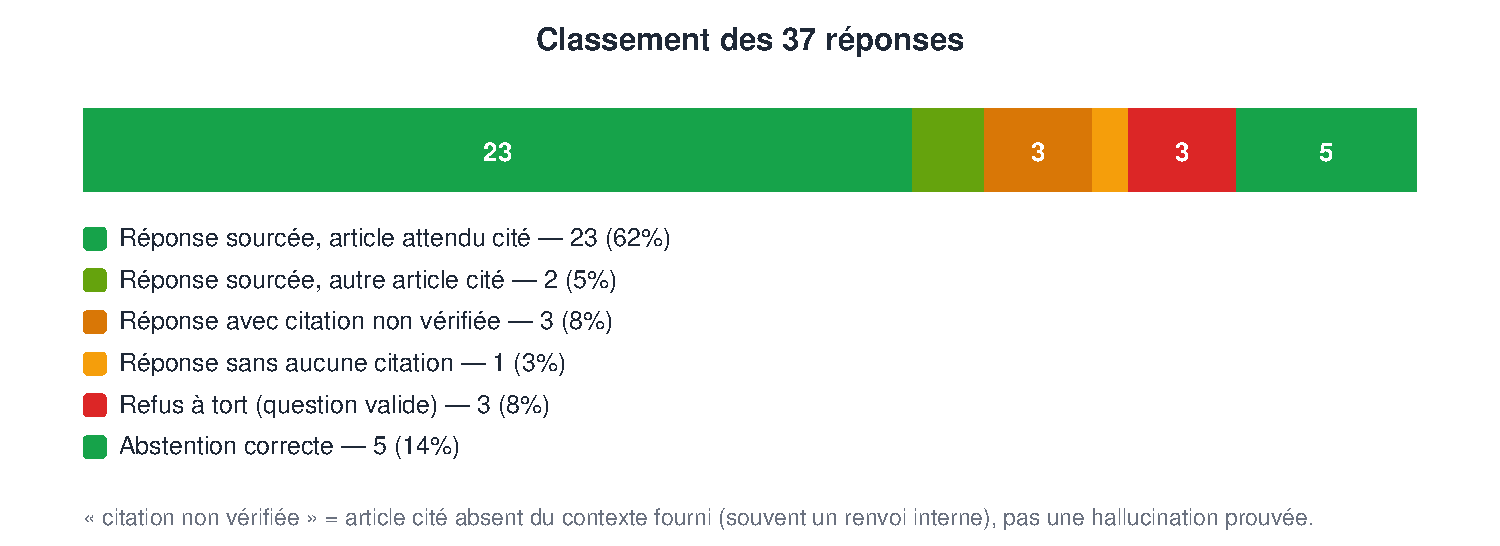
\includegraphics[width=\textwidth]{Figures/taxonomie-resultats.pdf}
    \caption{Répartition des 37 réponses par catégorie}
    \label{fig:taxonomie}
\end{figure}

La dernière ligne du tableau~\ref{tab:taxonomie} est la plus importante pour un outil juridique :
\textbf{aucune réponse n'a été produite sur un sujet absent du corpus}.

\subsection{Indicateurs de fiabilité}

\begin{itemize}
    \item \textbf{Citation systématique} : 97~\% des réponses citent au moins un article.
    \item \textbf{Vérification des citations} : 94~\% des articles cités figuraient effectivement
    dans le contexte fourni au modèle.
    \item \textbf{Abstention correcte} : 100~\% des questions hors périmètre ont été refusées.
\end{itemize}

\begin{figure}[H]
    \centering
    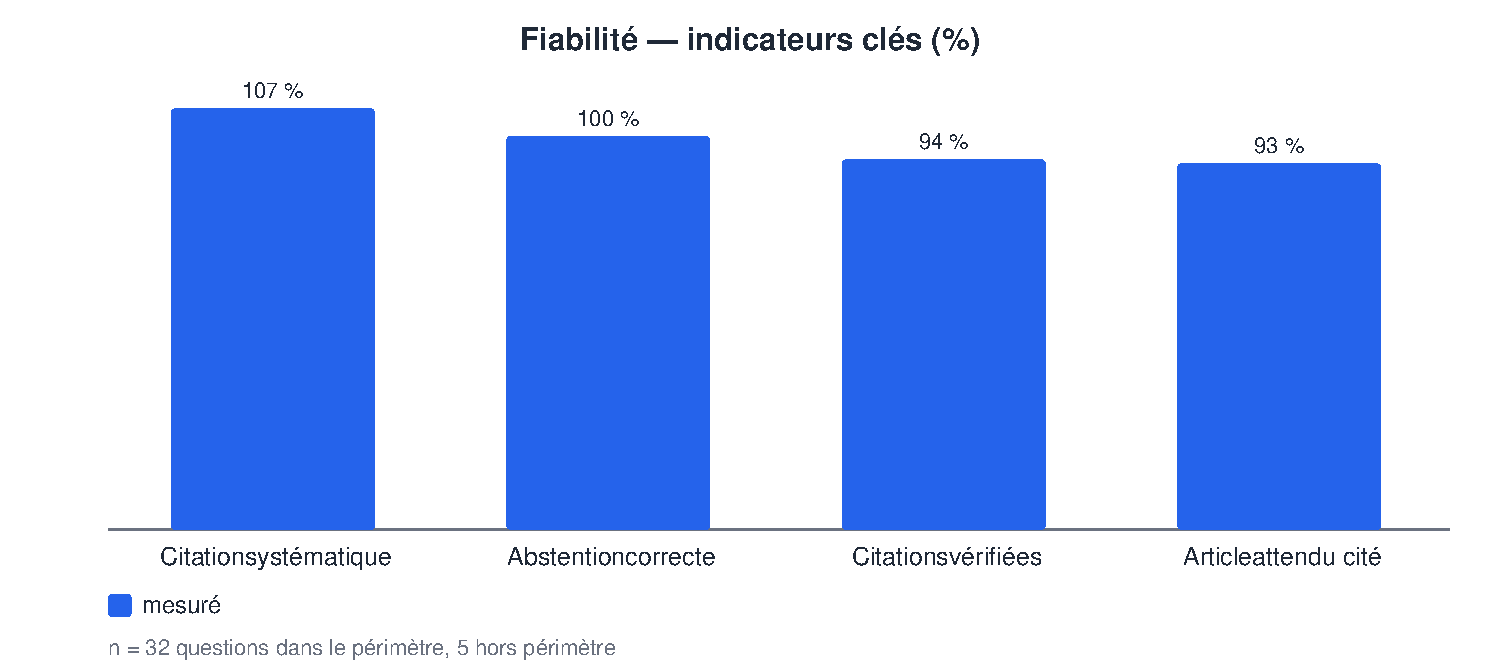
\includegraphics[width=\textwidth]{Figures/fiabilite-synthese.pdf}
    \caption{Indicateurs de fiabilité}
    \label{fig:fiabilite}
\end{figure}

Les citations restées « non vérifiées » sont, à l'examen, des \textbf{renvois internes} : le
texte d'un article fourni mentionne lui-même d'autres articles (« …dans les conditions prévues
par les articles 154 et 156 »), que le modèle reprend. Le contrôle signale ces numéros parce
qu'ils ne figurent pas dans le contexte ; il sur-signale volontairement, plutôt que de risquer de
manquer une véritable invention.

\section{Le garde-fou d'abstention}

\subsection{Calibration du seuil}

Le seuil d'abstention a été calibré empiriquement, non choisi arbitrairement. La mesure des
scores de recherche sur les deux populations de questions révèle trois bandes distinctes :

\begin{itemize}
    \item Questions de droit du travail : scores de \textbf{0{,}596} à \textbf{0{,}793}.
    \item Questions d'un \emph{autre domaine juridique} : environ 0{,}47 à 0{,}52 --- plus élevées
    que les précédentes car elles partagent le vocabulaire juridique français.
    \item Questions sans rapport avec le droit : \textbf{0{,}307} à environ 0{,}35.
\end{itemize}

\begin{figure}[H]
    \centering
    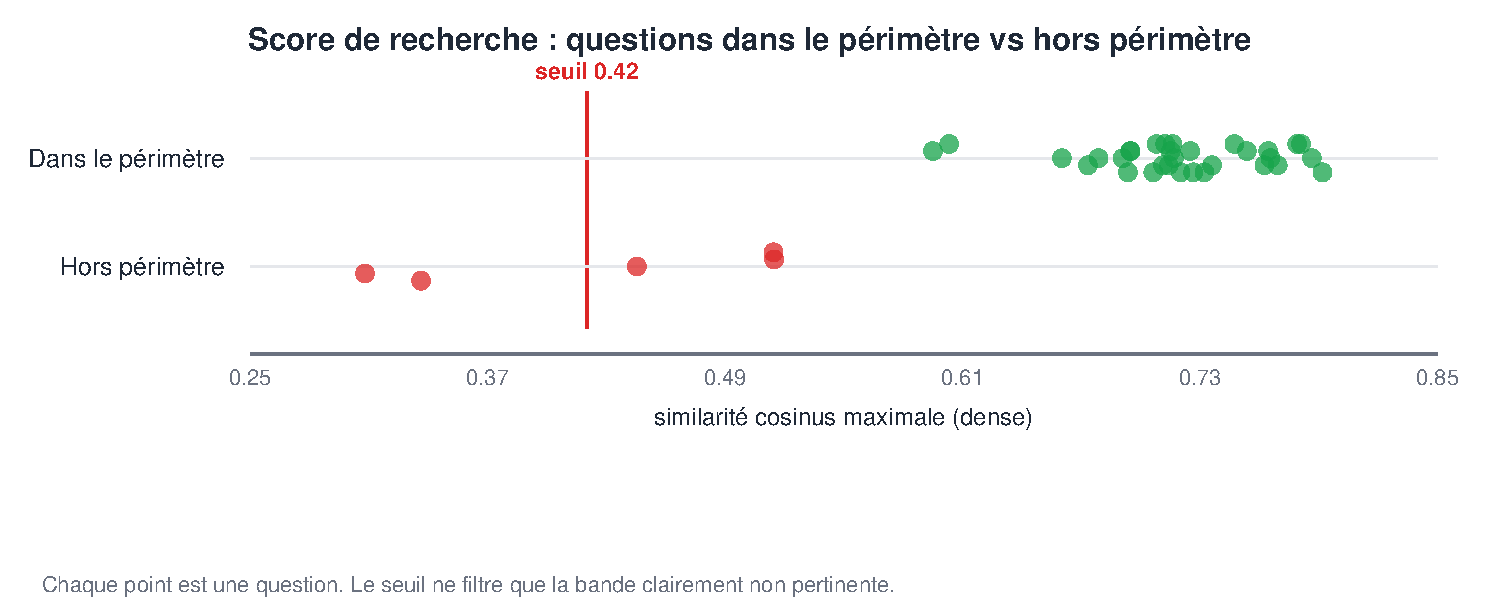
\includegraphics[width=\textwidth]{Figures/separation-abstention.pdf}
    \caption{Séparation des scores de recherche selon le périmètre de la question}
    \label{fig:separation}
\end{figure}

Ce constat a une conséquence de conception importante : \textbf{un seuil unique ne peut pas
séparer le droit du travail des autres domaines juridiques} --- et ne doit pas essayer. Le jour
où le corpus sera étendu à un second code, ces questions devront précisément devenir
répondables. Le seuil retenu (\textbf{0{,}42}) ne filtre donc que la bande clairement non
pertinente ; les questions juridiques hors corpus le franchissent et sont rattrapées par
l'abstention au niveau du prompt.

\subsection{Coût de l'abstention}

Trois questions valides sur 32 ont été refusées à tort. C'est le prix d'une abstention stricte,
et l'arbitrage est assumé : pour un outil juridique, un refus injustifié est préférable à une
réponse inventée. Cet équilibre reste néanmoins perfectible.

\section{Latence}

\begin{table}[H]
    \centering
    \begin{tabular}{|m{4.6cm}|m{2.2cm}|m{2.2cm}|m{2cm}|m{2cm}|}
        \hline
        \textbf{Étape} & \textbf{Médiane} & \textbf{Moyenne} & \textbf{p90} & \textbf{Max} \\
        \hline
        Recherche & 0{,}16 s & 0{,}17 s & 0{,}18 s & 0{,}46 s \\
        \hline
        Génération (modèle) & 3{,}28 s & 3{,}93 s & 7{,}23 s & 12{,}93 s \\
        \hline
        \textbf{Total avec génération} & \textbf{3{,}49 s} & 4{,}11 s & 7{,}48 s & 13{,}08 s \\
        \hline
        \textbf{Total, abstention} & \textbf{0{,}14 s} & 0{,}14 s & 0{,}14 s & 0{,}14 s \\
        \hline
    \end{tabular}
    \caption{Temps de réponse mesurés (37 questions, Mistral 7B en local)}
    \label{tab:latence}
\end{table}

\begin{figure}[H]
    \centering
    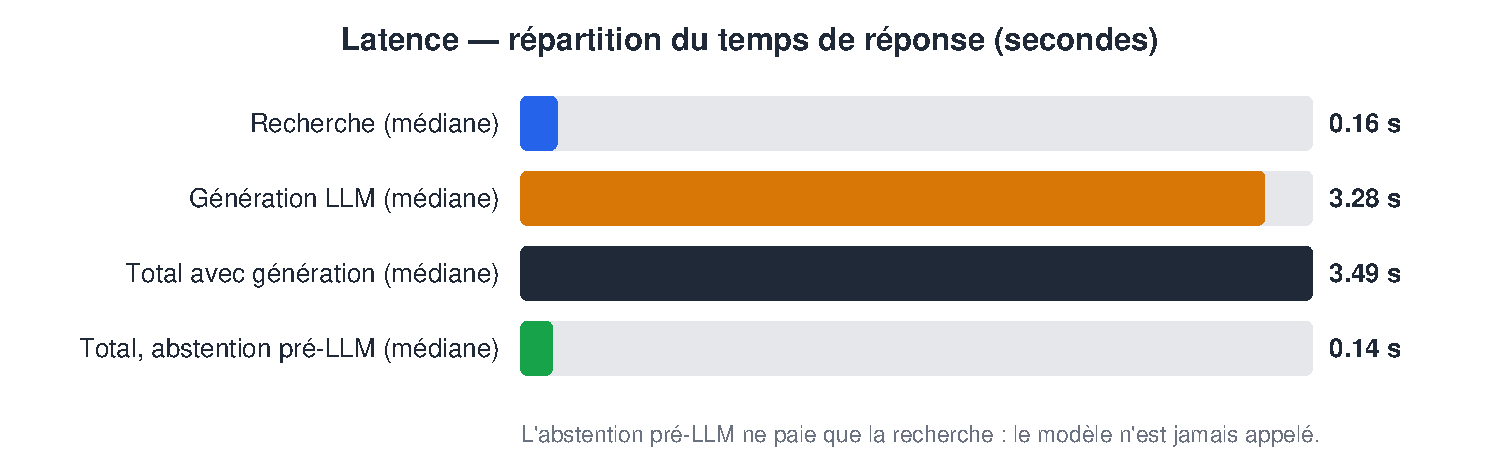
\includegraphics[width=\textwidth]{Figures/latence-repartition.pdf}
    \caption{Répartition du temps de réponse}
    \label{fig:latence}
\end{figure}

Deux observations méritent d'être relevées :

\paragraph{La recherche ne représente que 5~\% du temps total.}
L'ensemble de la chaîne de recherche --- vectorisation de la question, interrogation des deux
index, fusion --- coûte 0{,}16~seconde. Tout le reste est de l'inférence. Optimiser davantage la
recherche n'apporterait donc rien sur le temps de réponse perçu.

\paragraph{Le garde-fou divise le temps de réponse par 25.}
Une question hors périmètre reçoit sa réponse en 0{,}14~seconde contre 3{,}49~secondes pour une
réponse complète, puisque le modèle n'est jamais appelé. Le placement du garde-fou \emph{avant}
le modèle, décidé pour des raisons de fiabilité, produit ainsi un bénéfice de performance qui
n'était pas son objectif premier.

\section{Défaillance observée et corrigée}
\label{sec:hallucination}

L'évaluation a mis au jour une défaillance qui n'était pas apparue lors des tests manuels, et qui
mérite d'être rapportée en détail car elle constitue le mode d'échec le plus dangereux pour ce
type de système.

Interrogé sur la procédure de divorce --- question hors périmètre --- le modèle refusait
correctement, \emph{puis inventait une réponse complète} citant un « Code civil marocain (Loi
14-82) » et son « article 96 », en affirmant l'avoir consulté. Ces références n'existent pas : le
droit de la famille marocain relève de la Moudawana (loi 70-03), et aucun texte de ce type n'avait
été fourni au modèle.

Ce comportement --- reconnaître l'absence d'information puis produire malgré tout un contenu
inventé --- est plus trompeur qu'une invention franche : la prudence apparente du début de la
réponse renforce la crédibilité de ce qui suit.

La correction a consisté à interdire explicitement, dans le prompt système, toute mention d'un
numéro de loi ou d'article provenant d'un autre code. Une première version de cette règle s'est
révélée \textbf{trop stricte} : le taux d'abstention correcte est passé à 100~\%, mais les refus à
tort ont triplé. Une règle de rééquilibrage --- \emph{par défaut, réponds} --- a permis de
conserver le bénéfice sans le coût.

Cet épisode illustre l'intérêt d'un banc d'évaluation rejouable : sans lui, la sur-correction
serait passée inaperçue, le système paraissant simplement « plus prudent » alors qu'il devenait
moins utile.

\section{Limite de mesure assumée}

La vérification des citations contrôle qu'un article cité \textbf{figurait dans le contexte
fourni} --- pas qu'il \textbf{dise réellement} ce que la réponse lui attribue. Une réponse citant
un article réel tout en en déformant le contenu est comptée ici comme sourcée.

Détecter ce cas demanderait une vérification d'implication (\textit{entailment}) ou une relecture
humaine systématique. C'est hors du périmètre de ce stage, et le chiffre de 94~\% de citations
vérifiées doit être lu avec cette réserve : il mesure la \emph{traçabilité} des sources, non la
\emph{fidélité sémantique} des affirmations.

\newpage
\section*{Conclusion}

Le système atteint les objectifs de fiabilité fixés : citation quasi systématique, abstention
correcte sur l'intégralité des questions hors périmètre, et aucune réponse produite sur un sujet
absent du corpus. Deux résultats vont à l'encontre des attentes initiales --- la supériorité du
dense sur l'hybride, et l'existence d'une hallucination inter-codes invisible aux tests manuels
--- et n'ont pu être établis que grâce à une évaluation systématique et rejouable.
